\chapter{Relative entropy}
\lbl{ch:rel}
\index{relative entropy}

The notion of relative entropy allows us to compare two probability
distributions on the same space.  More specifically, for each pair of
probability distributions $\p, \vc{r}$ on the same finite set, there is
defined a real number $\relent{\p}{\vc{r}} \geq 0$, the entropy of $\p$
relative to $\vc{r}$.  It is zero just when $\p = \vc{r}$.  It extends the
definition of Shannon entropy, in the sense that the Shannon entropy of a
single distribution $\p$ on $\{1, \ldots, n\}$ is a function of
$\relent{\p}{\vc{u}_n}$, the entropy of $\p$ relative to the uniform
distribution.

Relative entropy goes by a remarkable number of names,%
%
\index{relative entropy!names for} 
%
attesting to its wide variety of interpretations and uses.  It is also
known as Kullback--Leibler information (as in \cite{ScheTS}, for instance),
Kullback--Leibler distance~\cite{CoTh1}, Kullback--Leibler
divergence~\cite{Joyc}, directed divergence~\cite{KullITS}, information
divergence~\cite{GrNi}, information deficiency~\cite{BJTV}, amount of
information~\cite{Reny}, discrimination information~\cite{KullKLD},
relative information~\cite{TaKu}, gain of information or information gain
(\cite{RenyPT}, Section~IX.4), discrimination distance~\cite{KantDDB}, and
error~\cite{Kerr}, among others.  This chapter provides multiple
explanations and applications of relative entropy, as well as a theorem
pinpointing what makes relative entropy uniquely useful.

Our first explanation of relative entropy is in terms of coding
(Section~\ref{sec:rel-coding}).  As we saw in Section~\ref{sec:ent-coding},
the Shannon entropy of $\p$ gives the average number of bits per
symbol needed to encode an alphabet with frequency distribution $\p$ in a
coding system optimized for that purpose.  In a similar sense,
$\relent{\p}{\vc{r}}$ measures the \emph{extra} number of bits per symbol
needed to encode an alphabet with frequencies $\p$ using a coding system
that was optimized for the frequency distribution $\vc{r}$.  In other
words, it is the penalty for using the wrong system.

The exponential of relative entropy is called relative diversity
(Section~\ref{sec:rel-div}).  Often we have a preconceived idea of what
an ordinary or default distribution of species is, and we judge how unusual
a community is relative to that expectation.  For instance, if we were
assessing the diversity of flowering plants in a particular region of
the island of Tasmania, we would naturally judge it by the standards of
Tasmania as a whole.  The relative diversity $\exp(\relent{\p}{\vc{r}})$
reflects the unusualness of a community with distribution $\p$ relative to
a reference distribution $\vc{r}$.

Section~\ref{sec:rel-misc} gives short accounts of roles played by relative
entropy in three other subjects.  In measure theory, we find that the
definition of relative entropy generalizes easily from finite sets to
arbitrary measurable spaces, while ordinary Shannon entropy does not.  The
slogan is: \emph{all%
%
\index{all entropy is relative} 
% 
entropy is relative}.  In geometry, although $\relent{-}{-}$ does not
define a distance function on the set $\Delta_n$ of distributions, it turns
out that infinitesimally, it behaves like the square of a distance.  We can
extend this infinitesimal metric to a global metric in the manner of
Riemannian geometry.  In statistics, the second argument $\vc{r}$ of
$\relent{\p}{\vc{r}}$ should be thought of as a prior\index{prior}, and
maximizing likelihood can be reinterpreted as minimizing relative entropy.
The concept of relative entropy also gives rise to the notions of Fisher
information and the Jeffreys prior, an objective prior distribution in the
sense of Bayesian statistics.

We finish the chapter with a characterization theorem for relative entropy
(Section~\ref{sec:rel-char}), which first appeared in~\cite{SCRE}.  Just as
for Faddeev's characterization of ordinary entropy, the main characterizing
property is a chain rule.  And just as for ordinary entropy, many
characterization theorems for relative entropy have previously been proved;
but the one presented here appears to be the simplest yet.



\section{Definition and properties of relative entropy}
\lbl{sec:rel-defn}


This short section presents the definition and basic properties of
relative entropy, without motivation for now.  The later sections provide
multiple interpretations of, and justifications for, the definition.

\begin{defn}
\lbl{defn:rel-ent}
Let $n \geq 1$ and $\vc{p}, \vc{r} \in \Delta_n$.  The
\demph{entropy%
%
\index{relative entropy} 
% 
of $\vc{p}$ relative to $\vc{r}$} is
% 
\begin{equation}
\lbl{eq:defn-rel-ent}
\relent{\vc{p}}{\vc{r}}
=
\sum_{i \in \supp(\p)} p_i \log \frac{p_i}{r_i}.
\end{equation}
% 
If there is some $i$ such that $p_i > 0 = r_i$ then
$\relent{\vc{p}}{\vc{r}}$ is defined to be $\infty$.
\end{defn}

In the literature, relative entropy is more often denoted by
$\reldiv{\vc{p}}{\vc{r}}$, but in this text, we reserve the letter $D$ for
measures of diversity.

\begin{example}
\lbl{eg:rel-ent-ufm}
Let $\p \in \Delta_n$.  Then
% 
\begin{align*}
\relent{\p}{\vc{u}_n}   &
=
\sum_{i \in \supp(\p)} p_i \log(np_i)   \\
&
=
\log n - H(\p)  \\
&
=
H(\vc{u}_n) - H(\p).
\end{align*}
% 
Thus, ordinary entropy is essentially a special case of relative entropy.
\end{example}

\begin{example}
\lbl{eg:rel-ent-large}
As well as sometimes taking the value $\infty$, relative entropy can take
arbitrarily large finite values (even for fixed $n$).  For instance, for $t
\in (0, 1)$, 
\[
\relEnt{\vc{u}_2}{(t, 1 - t)} 
=
\frac{1}{2} \log \frac{1}{2t} + \frac{1}{2} \log \frac{1}{2(1 - t)}
\to 
\infty
\]
as $t \to 0$.  
\end{example}

Unless $\vc{p} = \vc{r}$, there are some values of $i$ for which $p_i >
r_i$ and others for which $p_i < r_i$.  Hence, some of the summands
in~\eqref{eq:defn-rel-ent} are positive and others are negative.
Nevertheless:

\begin{lemma}
\lbl{lemma:rel-ent-pos-def}
$\relent{\vc{p}}{\vc{r}} \geq 0$, with equality if and only if $\vc{p} =
  \vc{r}$. 
\end{lemma}

\begin{proof}
If $p_i > 0 = r_i$ for some $i$ then $\relent{\vc{p}}{\vc{r}} = \infty$.
Suppose otherwise, so that $\supp(\p) \sub \supp(\vc{r})$.  Using
Lemma~\ref{lemma:log-concave},
% 
\begin{align*}
\relent{\vc{p}}{\vc{r}} &
=
- \sum_{i \in \supp(\p)} p_i \log \frac{r_i}{p_i}       \\
&
\geq    
- \log \Biggl( \sum_{i \in \supp(\p)} p_i \frac{r_i}{p_i} \Biggr)       \\
&
\geq
- \log \Biggl( \sum_{i \in \supp(\vc{r})} r_i \Biggr)   \\
&
=
- \log 1 
=
0,
\end{align*}
% 
with equality in the first inequality if and only if $r_i/p_i = r_j/p_j$
for all $i, j \in \supp(\p)$.  Equality holds in the second inequality if
and only if $\supp(\p) = \supp(\vc{r})$.  Hence for equality to hold
throughout, there must be some constant $\alpha$ such that $r_i = \alpha
p_i$ for all $i \in \supp(\p) = \supp(\vc{r})$.  But since $\sum_{i \in
  \supp(\p)} p_i = 1 = \sum_{i \in \supp(\vc{r})} r_i$, this forces $\alpha
= 1$ and so $\vc{p} = \vc{r}$.
\end{proof}

Lemma~\ref{lemma:rel-ent-pos-def} suggests that \emph{very} roughly
speaking, $\relent{\vc{p}}{\vc{r}}$ can be understood as a kind of
distance%
% 
\index{relative entropy!metric@as metric} 
% 
between $\vc{p}$ and $\vc{r}$.  However, relative entropy does not satisfy
the triangle inequality (Example~\ref{eg:rel-tri}).  Nor is it symmetric:%
% 
\index{relative entropy!asymmetry of}
% 
for as Examples~\ref{eg:rel-ent-ufm} and~\ref{eg:rel-ent-large} show,
$\relent{\p}{\vc{u}_2} \leq \log 2$ for all $\p \in \Delta_2$, whereas
$\relent{\vc{u}_2}{\p}$ can be arbitrarily large.  We will return to the
interpretation of relative entropy as a measure of distance in
Section~\ref{sec:rel-misc}.

We now list some of the basic properties of relative entropy.  Matters are
simplified if we restrict to just those pairs $(\vc{p}, \vc{r})$ such that
$\relent{\vc{p}}{\vc{r}} < \infty$.  For $n \geq 1$, write
% 
\begin{align*}
\lbl{p:An}
A_n     &
=
\{ (\vc{p}, \vc{r}) \in \Delta_n \times \Delta_n \such
r_i = 0 \implies p_i = 0 \}     \\
&
=
\{ (\vc{p}, \vc{r}) \in \Delta_n \times \Delta_n \such
\supp(\vc{p}) \sub \supp(\vc{r}) \}.
\end{align*}
% 
Then 
\[
\relent{\vc{p}}{\vc{r}} < \infty \iff (\vc{p}, \vc{r}) \in A_n.  
\]
So for each $n \geq 1$, we have the function
% 
\begin{equation*}
% \lbl{eq:restricted-rel-ent}
\begin{array}[c]{cccc}
\relent{-}{-}\from      &A_n            &\to    &\R    \\
                        &(\vc{p}, \vc{r})&\mapsto&\relent{\vc{p}}{\vc{r}}.
\end{array}
\end{equation*}
% 
This sequence of functions has the following properties, among others.
% 
\begin{description}
\item[Measurability%
% 
\index{measurability!relative entropy@of relative entropy}% 
\index{relative entropy!measurability of}
% 
in the second argument.]
For each fixed $\vc{p} \in \Delta_n$, the function
\[
\begin{array}{ccc}
\{ \vc{r} \in \Delta_n \such (\vc{p}, \vc{r}) \in A_n \}        &
\to     &
\R     \\
\vc{r}  &
\mapsto &
\relent{\vc{p}}{\vc{r}}
\end{array}
\]
is measurable.  Indeed, the function $\relent{-}{-} \from A_n \to \R$ is
continuous, but for the unique characterization of relative entropy proved
in Section~\ref{sec:rel-char}, measurability in the second argument is all
we will need.

\item[Permutation-invariance.]%
% 
\index{permutation-invariance}%
\index{relative entropy!permutation-invariance of} 
% 
The relative entropy $\relent{\p}{\vc{r}}$ is unchanged if the same
permutation is applied to the indices of both $\vc{p}$ and $\vc{r}$.  That
is,
\[
\relent{\p}{\vc{r}}
=
\relent{\p\sigma}{\vc{r}\sigma}
\]
for all $(\p, \vc{r}) \in A_n$ and permutations $\sigma$ of $\{1, \ldots,
n\}$, where
% 
\begin{equation}
\lbl{eq:p-perm}
\p\sigma = (p_{\sigma(1)}, \ldots, p_{\sigma(n)})
\end{equation}
% 
and similarly $\vc{r}\sigma$.  
% We use the term
% \demph{permutation-invariance} rather than `symmetry' to avoid confusion
% with the fact that $\relent{\p}{\vc{r}} \neq \relent{\vc{r}}{\p}$.

\item[Vanishing.]%
% 
\index{vanishing}%
\index{relative entropy!vanishing of}
% 
$\relent{\p}{\p} = 0$ for all $\p \in \Delta_n$.

\item[Chain rule.]
\index{chain rule!relative entropy@for relative entropy}%
\index{relative entropy!chain rule for}
Let $n, k_1, \ldots, k_n \geq 1$ and
\[
(\w, \widetilde{\w}) \in A_n, \  
\bigl(\p^1, \widetilde{\p}^1\bigr) \in A_{k_1}, \ 
\ldots, \ 
\bigl(\p^n, \widetilde{\p}^n\bigr) \in A_{k_n}.
\]
Then
% 
\begin{equation}
\lbl{eq:rel-ch}
\relEnt{\w \of (\p^1, \ldots, \p^n)}
{\widetilde{\w} \of (\widetilde{\p}^1, \ldots, \widetilde{\p}^n)}
=
\relent{\w}{\widetilde{\w}} + \sum_{i = 1}^n w_i
\relent{\p^i}{\widetilde{\p}^i}. 
\end{equation}
% 
This is a straightforward check, similar to
Proposition~\ref{propn:ent-chain}.  Note that
\[
\bigl(\w \of (\p^1, \ldots, \p^n),
\widetilde{\w} \of (\widetilde{\p}^1, \ldots, \widetilde{\p}^n)\bigr)
\in 
A_{k_1 + \cdots + k_n},
\]
so the relative entropy of this pair is guaranteed to be finite.

As a special case, relative entropy has a logarithmic property:
% 
\begin{equation}
\lbl{eq:rel-log}
\relent{\w \otimes \p}{\widetilde{\w} \otimes \widetilde{\p}}
=
\relent{\w}{\widetilde{\w}} + \relent{\p}{\widetilde{\p}}
\end{equation}
% 
for all $(\w, \widetilde{\w}) \in A_n$ and $(\p, \widetilde{\p}) \in A_k$.
This follows from the chain rule by taking $k_i = k$, $\p^i = \p$ and
$\widetilde{\p}^i = \widetilde{\p}$ for all $i \in \{1, \ldots, n\}$.  
\end{description}

Just as for ordinary entropy, different choices of the base of the
logarithm in the definition of relative entropy only change it by a
constant factor.  We will see in Section~\ref{sec:rel-char} that up to a
constant factor, the four properties just listed characterize relative
entropy uniquely.


\section{Relative entropy in terms of coding}
\lbl{sec:rel-coding}
\index{relative entropy!coding@and coding}

We have already interpreted Shannon entropy in terms of coding
(Section~\ref{sec:ent-coding}).  Here we do the same for relative entropy.  

To help our understanding, let us regard a probability distribution $\p \in
\Delta_n$ as the frequency distribution of the $n$ symbols in some human
language, which we call \demph{language%
%
\index{language p@language $\p$}
% 
$\p$}.  We make use of the convenient fiction introduced on
p.~\pageref{p:fiction}, imagining that there exists an ideal code for
language $\p$: a code whose average word length is exactly $\Hi(\p)$.  We
will suppose that the encoding is performed by a machine, called
\demph{machine%
%
\index{machine p@machine $\p$} 
% 
$\p$}.  Although most distributions $\p$ have no ideal code, one can come
arbitrarily close (as in Section~\ref{sec:ent-coding}), and this justifies
the use of ideal codes as an explanatory device.

For $\p \in \Delta_n$, the ordinary base~$2$ entropy
\[
\Hi(\p) = \sum_{i \in \supp(\p)} p_i \log_2 \frac{1}{p_i}
\]
satisfies
\[
\Hi(\p)
=
\text{no.\ bits/symbol to encode language } \p \text{ using machine } \p.
\]
Now let $\p, \vc{r} \in \Delta_n$, with $\p$ and $\vc{r}$ viewed as the
frequency distributions of two languages on the same set of symbols.  Write
\[
\relenti{\p}{\vc{r}}
=
\sum_{i \in \supp(\p)} p_i \log_2 \frac{p_i}{r_i}
=
\frac{\relent{\p}{\vc{r}}}{\log 2}
\ntn{relenti}
\]
for the base~$2$ relative entropy.  We will interpret
$\relenti{\p}{\vc{r}}$ in terms of languages $\p$ and $\vc{r}$ and machines
$\p$ and $\vc{r}$.

To do this, first consider the quantity
% 
% \begin{equation}
% \lbl{eq:crossenti}
\[
\crossenti{\p}{\vc{r}}
=
\sum_{i \in \supp(\p)} p_i \log_2 \frac{1}{r_i}.
\ntn{crossenti}
\]
% \end{equation}
% 
Here $\log_2(1/r_i)$ is the number of bits that machine $\vc{r}$ uses to
encode the $i$th symbol.  (Of course, this is not usually an integer, but
recall the comments on ideal codes on p.~\pageref{p:ideal}.)  Hence
\[
\crossenti{\p}{\vc{r}}
=
\text{no.\ bits/symbol to encode language } \p \text{ using machine } \vc{r}.
\]
This quantity $\crossenti{\p}{\vc{r}}$, or its base~$e$ analogue
% 
\begin{equation}
\lbl{eq:crossent}
\crossent{\p}{\vc{r}} 
= 
\sum_{i \in \supp(\p)} p_i \log \frac{1}{r_i}
=
\crossenti{\p}{\vc{r}}\cdot \log 2,
\end{equation}
% 
is the \demph{cross%
%
\index{cross entropy} 
% 
entropy} of $\p$ with respect to $\vc{r}$.

The relative, cross and ordinary entropies are related by the equation
% 
\begin{equation}
\lbl{eq:rco}
\relent{\p}{\vc{r}} = \crossent{\p}{\vc{r}} - H(\p).
\end{equation}
% 
Hence
% 
\begin{align*}
\relenti{\p}{\vc{r}}    &
=
\crossenti{\p}{\vc{r}} - \Hi(\p)        
\\
&
=
\text{no.\ bits/symbol to encode language } \p \text{ using machine }
\vc{r}  
\\
&
\phantom{= \mbox{}}
{} - \text{no.\ bits/symbol to encode language } \p 
\text{ using machine } \p.
\end{align*}
% 
So, for the task of encoding language $\p$, the relative entropy
$\relenti{\p}{\vc{r}}$ is the number of \emph{extra} bits needed if one
uses machine $\vc{r}$ instead of machine $\p$.  Machine $\p$ is ideal for
the job: it is optimized for exactly this purpose.  Relative entropy is,
then, the penalty for using the wrong machine.

This provides an intuitive explanation of why $\relent{\p}{\vc{r}}$ is
always nonnegative and why $\relent{\p}{\p} = 0$.  It also suggests why
relative entropy can be arbitrarily large, as in the following example.

\begin{examples}
\lbl{egs:relenti-large-sym}
\begin{enumerate}
\item
\lbl{eg:relenti-ls-large}
Consider an alphabet with $n = 2$ symbols.  Suppose that language $\p$ uses
the two symbols with equal frequency, and that in language $\vc{r}$ the
frequency distribution is $(2^{-1000}, 1 - 2^{-1000})$.  Then machine
$\vc{r}$ encodes the first symbol with a word of $1000$ bits.  Since
language $\p$ uses this symbol half the time, the average word length when
encoding language $\p$ using machine $\vc{r}$ is at least $500$ bits.  This
is drastically worse than when language $\p$ is encoded using the most
suitable machine, machine $\p$, which has an average word length of just
$1$ bit.  So the relative entropy $\relenti{\p}{\vc{r}}$ is at least $499$.

\item
The same example provides intuition for the fact that
\[
\relent{\p}{\vc{r}} \neq \relent{\vc{r}}{\p}.
\]
Machine $\p$ encodes the two symbols of the alphabet as the binary words
$0$ and $1$, of length $1$ each.  Hence the average number of bits used when
encoding language $\vc{r}$ (or indeed, any other language) in machine $\p$
is $1$.  So $\relenti{\vc{r}}{\p}$ is less than $1$, and is therefore much
smaller than the value of $\relenti{\p}{\vc{r}}$ derived
in~\bref{eg:relenti-ls-large}.
\end{enumerate}
\end{examples}

\begin{remark}
\index{cross entropy}
% 
The name `cross entropy' has a tangled history.  It was introduced by Jack
Good%
%
\index{Good, Jack} 
% 
in 1955 (\cite{GoodSTN}, Section~6), who defined it as in
equation~\eqref{eq:crossent} above and gave it its name.  But later, Good
used `cross entropy' as a synonym for relative entropy (\cite{GoodMEH},
p.~913), and others have done the same (Shore and Johnson~\cite{ShJo}, for
instance).  Nowadays the term is often used in the context of the cross
entropy method in operational research~\cite{DKMR}.  In the broadest terms,
this involves fixing a distribution $\vc{p}$ and minimizing
$\relent{\p}{\vc{r}}$, or equivalently $\crossent{\p}{\vc{r}}$, among all
$\vc{r}$ subject to certain constraints.  It makes no difference which one
minimizes, by equation~\eqref{eq:rco}.  From that point of view, the
concepts are essentially interchangeable, which has not helped to clarify
the terminological situation either.

This text uses the term with its original meaning, in part because relative
entropy already has an overabundance of synonyms.
\end{remark}

The chain rule for relative entropy (equation~\eqref{eq:rel-ch}) can also
be explained in terms of coding, as in the following example.

\begin{example}
\index{French language}%
\index{Swiss French}%
\index{Canadian French}
% 
In Example~\ref{eg:ent-french}, we interpreted the chain rule for ordinary
Shannon entropy in terms of letters and their accents in French.  There are
many dialects of French, using the same letters and accents but slightly
different vocabulary, hence slightly different frequency distributions of
both letters and accents.  Here we consider Swiss and Canadian French,
which for brevity we call just `Swiss' and `Canadian'.

Define distributions $\vc{w}, \twid{\vc{w}}, \p^i, \twid{\p}^i$ as follows:
%  
\begin{align*}
\vc{w} \in \Delta_{26}: &
\text{ frequency distribution of letters in Swiss}     \\
\twid{\vc{w}} \in \Delta_{26}:   &
\text{ frequency distribution of letters in Canadian}
\end{align*}
% 
and then
% 
\begin{align*}
\vc{p}^1 \in \Delta_3:  &
\text{ frequency distribution of accents on \as{a} in Swiss}      \\
\twid{\vc{p}}^1 \in \Delta_3:  &
\text{ frequency distribution of accents on \as{a} in Canadian}      \\
\vdots  \\
\vc{p}^{26} \in \Delta_1:  &
\text{ frequency distribution of accents on \as{z} in Swiss}      \\
\twid{\vc{p}}^{26} \in \Delta_1:  &
\text{ frequency distribution of accents on \as{z} in Canadian}.
\end{align*}
% 
So, recalling the convention that a `symbol' is a letter plus a (possibly
nonexistent) accent,
% 
\begin{align*}
\vc{w} \of \bigl(\vc{p}^1, \ldots, \vc{p}^{26}\bigr)      &
=
\text{frequency distribution of symbols in Swiss}  \\
\twid{\vc{w}} \of \bigl(\twid{\vc{p}}^1, \ldots, \twid{\vc{p}}^{26}\bigr)&
=
\text{frequency distribution of symbols in Canadian}.
\end{align*}
%
Now suppose that we encode Swiss using the Canadian machine.  How much
extra does this cost (in bits/symbol) compared to encoding Swiss using the
Swiss machine?

Since every symbol consists of a letter with an accent, we expect to have:
% 
\begin{multline}
\lbl{eq:relent-french}
\text{mean extra cost per symbol}
=\\
\text{mean extra cost per letter}
+
\text{mean extra cost per accent}.
\end{multline}
% 
The mean extra cost per symbol is
\[
\relEnti{\vc{w} \of \bigl(\vc{p}^1, \ldots, \vc{p}^{26}\bigr)}%
{\twid{\vc{w}} \of \bigl(\twid{\vc{p}}^1, \ldots, \twid{\vc{p}}^{26}\bigr)}.
\]
The mean extra cost per letter is
\[
\relenti{\vc{w}}{\twid{\vc{w}}}.
\]
The mean extra cost per accent is computed by conditioning on the letter
that it decorates.  Since it is Swiss rather than Canadian that we are
encoding, the probability of the $i$th letter occurring is $w_i$, so
the mean extra cost per accent is
\[
\sum_{i = 1}^{26} w_i \relEnti{\p^i}{\twid{\p}^i}.
\]
Hence the hoped-for equation~\eqref{eq:relent-french} predicts that
\[
\relEnti{\vc{w} \of \bigl(\vc{p}^1, \ldots, \vc{p}^{26}\bigr)}%
{\twid{\vc{w}} \of \bigl(\twid{\vc{p}}^1, \ldots, \twid{\vc{p}}^{26}\bigr)}
=
\relenti{\vc{w}}{\twid{\vc{w}}}
+
\sum_{i = 1}^{26} w_i \relEnti{\p^i}{\twid{\p}^i}.
\]
This is indeed true.  It is exactly the chain rule of
Section~\ref{sec:rel-defn}. 
\end{example}


\section{Relative entropy in terms of diversity}
\lbl{sec:rel-div}
\index{relative entropy!diversity@and diversity}


In Section~\ref{sec:ent-div}, we interpreted the exponential of Shannon
entropy as the diversity of a biological community.  Here we interpret the
exponential of relative entropy as a measure of how diverse or atypical one
community is when seen from the perspective of another.  This
interpretation elaborates on ideas of Reeve%
%
\index{Reeve, Richard} 
% 
et al.~\cite{HPD}.

As in Section~\ref{sec:ent-div}, we consider communities of individuals
drawn from $n$ species, whose relative abundances define a probability
distribution on the set $\{1, \ldots, n\}$. 

\begin{defn}
Let $n \geq 1$ and $\p, \vc{r} \in \Delta_n$.  The \demph{diversity of $\p$
  relative to $\vc{r}$%
%
\index{relative diversity} 
% 
(of order~$1$)} is 
\[
\reldiv{\p}{\vc{r}}
=
e^{\relent{\p}{\vc{r}}}
=
\prod_{i \in \supp(\p)} \biggl( \frac{p_i}{r_i} \biggr)^{p_i} 
\in 
[1, \infty].
\ntn{reldiv}
\]
\end{defn}

(We repeat the warning that although in the literature, the notation
$\reldiv{\p}{\vc{r}}$ is often used to mean relative \emph{entropy}, we
reserve the letter $D$ for diversity.)

By Lemma~\ref{lemma:rel-ent-pos-def}, $\reldiv{\p}{\vc{r}} \geq 1$, with
equality if and only if $\p = \vc{r}$.  

It is helpful to regard $\vc{r}$ as the distribution of a reference%
% 
\index{community!reference}%
\index{reference community}
% 
community (a community that one considers to be normal or the
default) and $\p$ as the distribution of the community in which we
are primarily interested.  As
we will see, $\reldiv{\p}{\vc{r}}$ measures how exotic or unusual this
other community is from the viewpoint of the reference community.

To explain this, it is helpful to begin with another quantity:
% 
\begin{defn}
Let $n \geq 1$ and $\p, \vc{r} \in \Delta_n$.  The 
\demph{cross%
%
\index{cross diversity} 
% 
diversity of $\p$ with respect to $\vc{r}$ (of order~$1$)} is
\[
\crossdiv{\p}{\vc{r}}
=
e^{\crossent{\p}{\vc{r}}}
=
\prod_{i \in \supp(\p)} 
\biggl( \frac{1}{r_i} \biggr)^{p_i}
\in
[1, \infty].
\ntn{crossdiv}
\]
\end{defn}

In Section~\ref{sec:ent-div}, the ordinary diversity of $\p$, 
\[
D(\p) = \prod_{i \in \supp(\p)} \biggl( \frac{1}{p_i} \biggr)^{p_i},
\]
was interpreted as follows: $1/p_i$ is the rarity\index{rarity} of the
$i$th species within the community, and $D(\p)$ is therefore the average
rarity of individuals in the community.  (In this case, `average' means
geometric mean.)
% 
Cross diversity can be understood in a similar way.  If we use the second
community $\vc{r}$ as our reference point~-- the community by which others
are to be judged~-- then we naturally take the rarity or
specialness\index{specialness} of the $i$th species to be $1/r_i$ rather
than $1/p_i$.  Thus, $\crossdiv{\p}{\vc{r}}$ is the average rarity of
individuals in the first community, seen from the viewpoint of the second.

Since
% 
\begin{equation}
\lbl{eq:rel-cross-div}
\reldiv{\p}{\vc{r}} 
=
\frac{\crossdiv{\p}{\vc{r}}}{D(\p)},
\end{equation}
% 
the relative diversity measures how much \emph{more} diverse the first
community looks from the viewpoint of the second than from the viewpoint of
itself.  Some examples illuminate this interpretation.

\begin{example}
\lbl{eg:rel-div-same}
We have $\reldiv{\p}{\p} = 1$, which is the minimal
possible value of relative diversity: any community perceives itself as
completely normal.
\end{example}

\begin{example}
\lbl{eg:rel-div-liz} 
% 
Let $\vc{p}$ and $\vc{r}$ be the relative abundance distributions of
reptiles in Portugal and Russia, respectively.  Geckos\index{geckos} are
commonplace in Portugal but rare in Russia.  Hence from the Russian
viewpoint, the ecology of Portugal seems exotic or atypical, in this
respect at least.

Mathematically, there are several values of $i$ (corresponding to species
of gecko) such that $r_i$ is small but $p_i$ is not.  This means
that the cross diversity contains some large factors, $(1/r_i)^{p_i}$, and
the relative diversity also contains some large factors, $(p_i/r_i)^{p_i}$.
Thus, both the cross diversity $\crossdiv{\p}{\vc{r}}$ and the relative
diversity $\reldiv{\p}{\vc{r}}$ are large, regardless of the diversity
$D(\p)$ of reptiles in Portugal.
\end{example}

\begin{example}
Taking the previous example to the extreme, if one or more species is
present in the test community $\vc{p}$ but absent in the reference
community $\vc{r}$ then $\reldiv{\p}{\vc{r}} = \infty$.
\end{example}

\begin{example}
\lbl{eg:rel-div-ufm} 
% 
Suppose now that we judge communities from the
reference point of a community with a uniform distribution.  (This is in
some sense the canonical choice of reference, and is the one produced by
the maximum entropy method of statistics~\cite{JaynWDWS,BuMa}.)  The
cross diversity $\crossdiv{\p}{\vc{u}_n}$ is equal to $n$, regardless of
$\p$.  Hence equation~\eqref{eq:rel-cross-div} gives
% 
\begin{equation}
\lbl{eq:rel-div-ufm}
\reldiv{\p}{\vc{u}_n}
=
\frac{n}{D(\p)}.
\end{equation}
% 
This is also the exponential of the equation
\[
\relent{\p}{\vc{u}_n} = \log n - H(\p)
\]
derived in Example~\ref{eg:rel-ent-ufm}.

Equation~\eqref{eq:rel-div-ufm} implies that for a fixed number of species,
the diversity of a community relative to the uniform distribution is
inversely proportional to the intrinsic diversity of the community itself.
From the viewpoint of a community in which all $n$ species are balanced
equally, any variation from this balance looks unusual~-- and the more
unbalanced, the more unusual.  

As an illustration of the general point, house sparrows\index{sparrows} are
common throughout Britain, but a region of the country in which the
\emph{only} birds\index{birds} were house sparrows would be highly unusual.
Correspondingly, the relative diversity $\reldiv{\p}{\vc{r}}$ of that
region relative to the country would be high, even though the intrinsic
diversity $D(\p)$ of the region would take the minimum possible value, $1$.

By equation~\eqref{eq:rel-div-ufm} and Lemma~\ref{lemma:div1-max-min},
$\reldiv{\p}{\vc{u}_n}$ takes its minimal value, $1$, when $\vc{p} =
\vc{u}_n$.  It takes its maximal value, $n$, when
\[
\p = (0, \ldots, 0, 1, 0, \ldots, 0).
\]
That is, from the viewpoint of a completely balanced community, the most
unusual possible community is one consisting of a single species.
\end{example}

Often, we want to assess a community from the viewpoint of a larger
community that \emph{contains} it.  For instance, we are more likely to
study the diversity of plankton in the eastern Mediterranean Sea with reference
to the Mediterranean as a whole than with reference to the Arctic Ocean.

Consider, then, an ecological community with relative abundance
distribution $\vc{r} \in \Delta_n$, and a subcommunity consisting of some
of its organisms.  Write $\pi_i$ for the proportion of the community
consisting of individuals that belong to both the subcommunity and the
$i$th species.  Then $0 \leq \pi_i \leq r_i$.  The proportion of the whole
community made up by the subcommunity is $w = \sum \pi_i \leq 1$, and
the relative abundance distribution of the subcommunity is
\[
\p = (\pi_1/w, \ldots, \pi_n/w) \in \Delta_n.
\]
The inequality $\pi_i \leq r_i$ gives $w p_i \leq r_i$, or equivalently,
% 
\begin{equation}
\lbl{eq:sc-bd}
\frac{p_i}{r_i} \leq \frac{1}{w},
\end{equation}
% 
for all $i \in \supp(\vc{r})$.  Hence
\[
\reldiv{\p}{\vc{r}}
=
\prod_{i \in \supp(\p)} \biggl( \frac{p_i}{r_i} \biggr)^{p_i}
\leq
\prod_{i \in \supp(\p)} \biggl( \frac{1}{w} \biggr)^{p_i}
=
\frac{1}{w},
\]
giving
% 
\begin{equation}
\lbl{eq:rel-div-sc-bounds}
1 \leq \reldiv{\p}{\vc{r}} \leq \frac{1}{w}.
\end{equation}
% 
We now consider cases in which these bounds are attained.

\begin{examples}
\lbl{egs:rel-div-sc}
\begin{enumerate}
\item 
\lbl{eg:rel-div-sc-min}
By Lemma~\ref{lemma:rel-ent-pos-def}, $\reldiv{\p}{\vc{r}}$ attains its
lower bound of $1$ precisely when $\p = \vc{r}$.  This means that the
subcommunity is exactly typical or representative of the larger community;
it is minimally unusual.

\item
\lbl{eg:rel-div-sc-max}
% 
The maximum $\reldiv{\p}{\vc{r}} = 1/w$ in~\eqref{eq:rel-div-sc-bounds} is
attained when $r_i = w p_i$ for all $i \in \supp(\p)$.  In the notation
above, this is equivalent to $\pi_i = r_i$ for all $i \in \supp(\p)$.  In
other words, the subcommunity is \demph{isolated}\index{isolated}: the
species occurring in the subcommunity occur nowhere else in the community.

If the isolated subcommunity is very small then its species distribution
appears highly unusual from the viewpoint of the whole community, and
correspondingly $\reldiv{\p}{\vc{r}} = 1/w$ is large.  But if, say, the
isolated subcommunity makes up $90\%$ of the whole community, then from the
viewpoint of the whole, the ecology of the subcommunity looks very typical.
So, it is intuitively reasonable that $\reldiv{\p}{\vc{r}} = 1/0.9$ is
close to the minimal possible value of $1$ .
\end{enumerate}
\end{examples}

The difference between relative diversity and cross diversity is
illustrated by the case of a uniform reference community
(Example~\ref{eg:rel-div-ufm}) and by the following example.

\begin{example}
\lbl{eg:three-scs} 
Consider a community with species distribution $\vc{r}$, containing a
subcommunity with species distribution $\vc{q}$, which in turn contains a
subcommunity with species distribution $\vc{p}$
(Figure~\ref{fig:three-scs}).
% 
\begin{figure}
\centering
\lengths
\begin{picture}(120,30)
\cell{60}{15}{c}{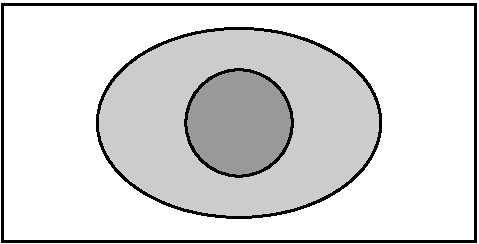
\includegraphics[height=30\unitlength]{nestedm}}
\cell{63}{18}{c}{$\vc{p}$}
\cell{71.5}{21}{c}{$\vc{q}$}
\cell{86}{26}{c}{$\vc{r}$}
\end{picture}
\caption{The three communities of Example~\ref{eg:three-scs}.}
\lbl{fig:three-scs}
\end{figure}
% 
Suppose that the two subcommunities consist only of species that are rare
in the whole community, with $r_i = 1/100$ for all $i \in \supp(\vc{q})$.
The larger subcommunity consists of $50$ such species, and the smaller of
just one. 

For the smaller subcommunity,
\[
D(\p) = 1,
\quad
\crossdiv{\p}{\vc{r}} = 100,
\quad
\reldiv{\p}{\vc{r}} = 100.
\]
Indeed, $D(\p) = 1$ since the subcommunity contains just one species. For
the cross diversity, $1/r_i = 100$ for all $i \in \supp(\p)$, and
$\crossdiv{\p}{\vc{r}}$ is the geometric mean of $1/r_i$ over $i \in
\supp(\p)$, so $\crossdiv{\p}{\vc{r}} = 100$.  Then $\reldiv{\p}{\vc{r}} =
100/1 = 100$.

For the larger subcommunity,
\[
D(\vc{q}) = 50,
\quad
\crossdiv{\vc{q}}{\vc{r}} = 100,
\quad
\reldiv{\vc{q}}{\vc{r}} = 2,
\]
by a similar argument.  

This can be understood as follows.  From the viewpoint of the whole
community, the average rarity of the individuals in either subcommunity
is~$100$.  This is why both have a cross diversity of~$100$.  But the
larger subcommunity looks less unusual than the smaller one, because it
occupies more of the community and therefore resembles it more closely.
This is why the relative diversity of the larger subcommunity is lower.
\end{example}

\begin{remark}
\lbl{rmk:abg-rel} 
In ecology, there are concepts of alpha-\index{alpha-diversity},
beta-\index{beta-diversity} and gamma-diversity\index{gamma-diversity}.
% 
\index{diversity!partitioning of}%
\index{partitioning of diversity}
%
The quantities $D(\p)$, $\reldiv{\p}{\vc{r}}$ and $\crossdiv{\p}{\vc{r}}$
are, respectively, kinds of alpha-, beta- and gamma-diversities, and
equation~\eqref{eq:rel-cross-div} is a version of the equation $\beta =
\gamma/\alpha$ that appears in the ecological literature (beginning with
Whittaker~\cite{WhitVSM},%
%
\index{Whittaker, Robert}
%
p.~321).

However, $D(\p)$, $\reldiv{\p}{\vc{r}}$ and $\crossdiv{\p}{\vc{r}}$ are
somewhat different from \mbox{alpha-,} beta- and gamma-diversity as usually
construed.  In the traditional ecological framework, a large community is
divided into a number of subcommunities, alpha-diversity is some kind of
average of the intrinsic diversities of the subcommunities, beta-diversity
is a measure of the variation between the subcommunities, and
gamma-diversity is, simply, the diversity of the whole.  Here,
non-traditionally, our beta-diversity (the relative diversity
$\reldiv{\p}{\vc{r}}$) and our gamma-diversity (the cross diversity
$\crossdiv{\p}{\vc{r}}$) express properties of an \emph{individual}
subcommunity with reference to the larger community.
% 
This is one of the innovations introduced in recent work of Reeve%
%
\index{Reeve, Richard} 
% 
et al.~\cite{HPD}, explored in depth in Chapter~\ref{ch:mm}.
\end{remark}


\section{Relative entropy in measure theory, geometry and statistics}
\lbl{sec:rel-misc}
\index{relative entropy!measure theory@and measure theory}%
\index{relative entropy!geometry@and geometry}%
\index{relative entropy!statistics@and statistics}

Here we give brief interpretations of relative entropy as seen from
specific standpoints in these three subjects.  


\subsection*{Measure theory}


Let us attempt to generalize the notion of Shannon entropy from probability
distributions on a finite set to probability measures on an arbitrary
measurable space $\Omega$.  Starting from the definition
\[
H(\p) = - \sum_{i \in \supp(\p)} p_i \log p_i
\]
for finite sets, and reasoning purely formally, one might try to define the
entropy%
%
\index{entropy!measure space@on measure space} 
% 
of a probability measure $\nu$ on $\Omega$ as
\[
H(\nu) = - \int_\Omega (\log \nu) \dee\nu.
\]
But this makes no sense, since there is no such function as `$\log \nu$'.

However, \emph{relative} entropy generalizes easily.  Indeed, given
probability measures $\nu$ and $\mu$ on $\Omega$, the
\demph{entropy of $\nu$ relative to $\mu$} is defined as
% 
\begin{equation}
\lbl{eq:rel-ent-meas}
\relent{\nu}{\mu}
=
\int_\Omega \log \biggl( \frac{d\nu}{d\mu} \biggr) \dee\nu
\in
[0, \infty],
\end{equation}
% 
where $d\nu/d\mu$ is
the Radon--Nikodym derivative.  (If $\nu$ is not absolutely
continuous with respect to $\mu$ then $d\nu/d\mu$ sometimes takes the value
$\infty$; but as in the finite case, we allow $\infty$ as a relative
entropy.)  

\begin{examples}
\lbl{egs:relent-meas}
\begin{enumerate}
\item
\lbl{eg:rm-dens}
Fix a measure $\lambda$ on $\Omega$, and take measures $\nu$ and $\mu$ on
$\Omega$ with densities $p$ and $r$ with respect to $\lambda$.  Thus, $d\nu
= p \dee\lambda$, $d\mu = r\dee\lambda$, and $d\nu/d\mu = p/r$.  It follows
that
% 
\begin{equation*}
% \lbl{eq:rel-ent-dens}
\relent{\nu}{\mu}
=
\int_{\supp(p)} p \log \biggl(\frac{p}{r}\biggr) \dee\lambda.
\end{equation*}
% 
Provided that the choice of reference measure $\lambda$ is understood,
$\relent{\nu}{\mu}$ can be written as $\relent{p}{r}$.

\item
In particular, when $\Omega$ is a finite set with counting measure
$\lambda$, we recover Definition~\ref{defn:rel-ent}.
\end{enumerate}
\end{examples}

The measure-theoretic viewpoint also explains some earlier notation.  On
p.~\pageref{p:An}, we introduced the set $A_n$ of pairs $(\vc{p}, \vc{r})$
of probability distributions on $\{1, \ldots, n\}$ such that
$\relent{\p}{\vc{r}} < \infty$.  Regarding $\vc{p}$ and $\vc{r}$ as
measures on $\{1, \ldots, n\}$, the set $A_n$ consists of exactly the pairs
such that $\vc{p}$ is absolutely continuous with respect to $\vc{r}$.

The slogan
% 
\slogan{all entropy is relative}%
\index{all entropy is relative}
% 
is partly justified by the fact just established: relative entropy makes
sense in a wide measure-theoretic context in a way that ordinary entropy
does not.  A different justification is given in
Section~\ref{sec:all-ent-rel}.

There is, nevertheless, a useful concept of the entropy of a probability
distribution on Euclidean space.  Indeed, the
\demph{differential entropy}%
%
\index{entropy!differential}%
\index{differential entropy}
% 
of a probability density function $f$ on $\R^n$ is defined as
% 
% \begin{equation}
% \lbl{eq:ent-Rn}
\[
H(f)
=
-\int_{\supp(f)} f(x) \log f(x) \dx,
\]
% \end{equation}
% 
and it is a fundamental fact that among all density functions with a given
mean and variance, the one with the maximal entropy is the
normal%
%
\index{normal distribution} 
% 
distribution.  (This fact is closely related
to the central%
%
\index{central limit theorem} 
% 
limit theorem, as explained in Johnson~\cite{JohnITC}, for instance.)
However, $H(f)$ is still a kind of relative entropy, since the integration
takes place with respect to Lebesgue measure $\lambda$.  Writing $\nu =
f\dee\lambda$ for the probability measure corresponding to the density $f$,
we have $f = d\nu/d\lambda$, hence
\[
H(f)
=
- \int \log \biggl( \frac{d\nu}{d\lambda} \biggr) \dee\nu.
\]
Formally, the right-hand side is the negative of the expression for
$\relent{\nu}{\lambda}$ given by equation~\eqref{eq:rel-ent-meas}, even
though $\lambda$ is not a \emph{probability} measure.


\subsection*{Geometry}
\index{relative entropy!metric@as metric}

We have tentatively evoked the idea that $\relent{\p}{\vc{r}}$ is some kind
of measure of distance, difference or divergence between the probability
distributions $\p$ and $\vc{r}$, and it is true that $\relent{\p}{\vc{r}}
\geq 0$ with equality if and only if $\p = \vc{r}$.  However, we have also
seen that relative entropy does not have one of the standard properties of
a distance function:
\[
\relent{\p}{\vc{r}} \neq \relent{\vc{r}}{\p}.
% 
\index{relative entropy!asymmetry of}
\]
If that were the only problem, it would not be so bad: for as Lawvere,%
% 
\index{Lawvere, F. William}
% 
Gromov,%
% 
\index{Gromov, Misha} 
% 
and others have argued (\cite{LawvMSG}, p.~138--139
and~\cite{GromMSR}, p.~xv), and as anyone who has walked up and down a
hill\index{hill} 
already knows, there are useful notions of distance%
% 
\index{metric!nonsymmetric} 
% 
that are not symmetric.  A more serious problem is that relative entropy
fails the triangle inequality:%
% 
\index{relative entropy!triangle inequality@and triangle inequality}

\begin{example}
\lbl{eg:rel-tri}
Define $\p, \vc{q}, \vc{r} \in \Delta_2$ by 
\[
\vc{p} = (0.9, 0.1),
\quad
\vc{q} = (0.2, 0.8),
\quad
\vc{r} = (0.1, 0.9).
\]
Then
\[
\relent{\vc{p}}{\vc{q}}
+
\relent{\vc{q}}{\vc{r}}
=
1.190\ldots
<
1.757\ldots
=
\relent{\vc{p}}{\vc{r}}.
\]
\end{example}

So, relative entropy only crudely resembles a distance function or metric
in the sense of metric spaces.

However, it is a highly significant fact that the \emph{square root} of
relative entropy is an \emph{infinitesimal} distance on the set of
probability distributions.  We explain this twice: first informally, then
in the language of Riemannian geometry.

Informally, let $\p \in \Delta_n^\circ$, and consider the relative entropy 
\[
\relent{\p + \vc{t}}{\vc{p}}
\]
for $\vc{t} \in \R^n$ close to $\vc{0}$ such that $\sum t_i = 0$.  (Then
$\p + \vc{t} \in \Delta_n^\circ$.)  We can expand $\relent{\p +
  \vc{t}}{\vc{p}}$ as a Taylor series in $t_1, \ldots, t_n$.  Since
$\relent{\p + \vc{t}}{\p}$ attains its minimum of $0$ at $\vc{t} = \vc{0}$,
the constant term in the Taylor expansion is $0$ and the terms in $t_1,
\ldots, t_n$ also vanish.  A straightforward calculation shows that, in
fact,
\[
\relent{\p + \vc{t}}{\p} 
=
\sum_{i = 1}^n \frac{1}{2p_i} t_i^2
+ \text{higher order terms}.
\]
Thus, up to a different scale factor $1/2p_i$ in each coordinate, relative
entropy locally resembles the square of Euclidean distance.  The same
is true with the arguments reversed:
\[
\relent{\p}{\p + \vc{t}}
=
\sum_{i = 1}^n \frac{1}{2p_i} t_i^2
+ \text{higher order terms}.
\]
So although $\relent{-}{-}$ is not symmetric%
% 
\index{relative entropy!asymmetry of} 
% 
in its two arguments, it is infinitesimally so, to second order.

These formulas suggest that we regard the square root of relative entropy,
rather than relative entropy itself, as a metric.  But again, it is not a
metric in the sense of metric spaces, because it fails the triangle%
%
\index{relative entropy!triangle inequality@and triangle inequality}
% 
inequality.  The same $\p$, $\vc{q}$ and $\vc{r}$ as in
Example~\ref{eg:rel-tri} provide a counterexample:
\[
\sqrt{\relent{\vc{p}}{\vc{q}}}
+
\sqrt{\relent{\vc{q}}{\vc{r}}}
=
1.281\ldots
<
1.325\ldots
=
\sqrt{\relent{\vc{p}}{\vc{r}}}.
\]
% 
% Gnuplot code:
% 
% gnuplot> h(a,b,x,y) = sqrt(a*log(a/x) + b*log(b/y))
% gnuplot> f(a,x) = h(a,1-a,x,1-x)
% gnuplot> print f(.9,.2) + f(.2,.1) 
% 1.28110589114833
% gnuplot> print f(.9,.1)
% 1.3258128306322
% 

Nevertheless, $\sqrt{\relent{-}{-}}$ can successfully be used as an
\emph{infinitesimal}%
%
\index{infinitesimal metric} 
% 
metric.  Still speaking informally, the process is as follows.

Suppose that we are given a set $X \sub \R^n$ and a nonnegative real-valued
function $\delta$ defined on all pairs of points of $X$ that are
sufficiently close together. Then under suitable hypotheses on $\delta$, we
can define a metric $d$ on $X$.  First, define the length of any path
$\gamma$ in $X$ by finite approximations: plot a large number of
close-together points $\vc{x}_0, \ldots, \vc{x}_m$ along $\gamma$, use
$\sum_{r = 1}^m \delta(\vc{x}_{r - 1}, \vc{x}_r)$ as an approximation to
the length of $\gamma$, then pass to the limit.  The distance $d(\vc{x},
\vc{y}) \in [0, \infty]$ between two points $\vc{x}, \vc{y} \in X$ is
defined as the length of a shortest path between $\vc{x}$ and $\vc{y}$.
This $d$ is a metric in the sense of metric spaces.

Applied when $X = \Delta_n^\circ$ and $\delta = \sqrt{\relent{-}{-}}$, this
process gives a new metric $d$\ntn{dF1}%
%
\index{simplex!metric on} 
% 
on the simplex.  `Have you ever seen anything like that?'\ asked Gromov%
% 
\index{Gromov, Misha} 
% 
(\cite{GromSS1}, Section~2).  As it turns out, $d$ is not so exotic.  Let
\[
S^{n - 1} = \Bigl\{ \vc{x} \in \R^n \such \sum x_i^2 = 1 \Bigr\}
\]
denote the unit $(n - 1)$-sphere.  It carries the geodesic metric $d_{S^{n
    - 1}}$, in which $d_{S^{n - 1}}(\vc{x}, \vc{y})$ is the length of a
shortest path between $\vc{x}$ and $\vc{y}$ on the sphere (an arc of a
great circle).  Any distribution $\p \in \Delta_n^\circ$ has a
corresponding point $\sqrt{\p} = (\sqrt{p_1}, \ldots, \sqrt{p_n})$ on $S^{n
  - 1}$.  And as we will see, the metric $d$ on $\Delta_n^\circ$ satisfies
\[
d(\vc{p}, \vc{r}) 
= 
\sqrt{2} d_{S^{n - 1}}\bigl(\sqrt{\vc{p}}, \sqrt{\vc{r}}\bigr)
\]
($\p, \vc{r} \in \Delta_n^\circ$).  So when the simplex is equipped with
this distance $d$, it is isometric to a subset of the sphere of radius
$\sqrt{2}$.  With different constant factors, $d(\p, \vc{r})$ is known
as the Fisher%
%
\index{Fisher, Ronald!distance} 
% 
distance or Bhattacharyya%
%
\index{Bhattacharyya angle} 
% 
angle between $\p$ and $\vc{r}$, as detailed below.

We now sketch the precise development.  The story told here is the
beginning of the subject of information%
%
\index{information geometry}
% 
geometry, and we refer to the literature in that subject for details of
what follows.  The books by Ay, Jost, L{\^e} and
Schwachh{\"o}fer~\cite{AJLS} and Amari~\cite{AmarIGA} are comprehensive
modern introductions to information geometry.  Other important sources are
the earlier book of Amari and Nagaoka~\cite{AmNa}, the foundational 1983
paper of Amari~\cite{AmarFIG}, and the 1987 articles of
Lauritzen~\cite{Laur} and Rao~\cite{RaoDMP}.  The idea of converting an
infinitesimal distance-like function on a manifold into a genuine distance
function is developed systematically in Eguchi's theory of contrast
functions~\cite{EgucDGA,EgucGMC}, a summary of which can be found in
Section~3.2 of~\cite{AmNa}.

Let $M = (M, g)$ be a Riemannian%
%
\index{Riemannian manifold} 
% 
manifold, and write $d$ for its geodesic distance function.  (We
temporarily adopt the Riemannian geometers' practice of using \dmph{metric}
to mean a Riemannian metric, and \dmph{distance} for a metric in the sense
of metric spaces.)  For each point $p \in M$, we have the function
\[
d(-, p)^2 \from M \to \R.
\]
It takes its minimum value, $0$, at $p$, and is smooth on a neighbourhood
of $p$.  We can therefore take its Hessian\index{Hessian} (with respect to
the Levi-Civita connection) at any point $x$ near $p$, giving a bilinear
form
\[
\Hess_x \bigl( d(-, p)^2 \bigr)
\]
on the tangent space $T_x M$.  In particular, we can take $x = p$, giving a
bilinear form on $T_p M$.  But of course, we already have another bilinear
form on $T_p M$, the Riemannian metric $g_p$ at $p$.  And up to a
constant factor, the two forms are equal:
% 
\begin{equation}
\lbl{eq:loc-glob}
g_p
=
\frac{1}{2}
\Hess_p \bigl( d(-, p)^2 \bigr).
\end{equation}
% 
This equation expresses the Riemannian
metric in terms of the geodesic distance (together with the connection).
That is, it expresses infinitesimal distance in terms of global distance.

(Equation~\eqref{eq:loc-glob} is proved by an elementary calculation,
although it is not often stated directly in the literature.  It can be derived
from more sophisticated results such as Theorem~6.6.1 of
Jost~\cite{JostRGG}, by taking the limit as $x \to p$ there, or
equation~(5) in Supplement~A of Pennec~\cite{PennBSA}.)

The idea now is that given any manifold $M$ with connection and any
function $\delta \from M \times M \to \R$ with primitive distance-like
properties, we can define a Riemannian metric $g$ on $M$ by
% 
\begin{equation}
\lbl{eq:loc-glob-fake}
g_p
=
\frac{1}{2}
\Hess_p \bigl( \delta(-, p)^2 \bigr)
\end{equation}
% 
($p \in M$).  Then, in turn, $g$ gives rise to a geodesic distance function
$d$ on $M$.  So, starting from a distance-like function $\delta$, we will
have derived a \emph{genuine} distance function $d$.  By
equations~\eqref{eq:loc-glob} and~\eqref{eq:loc-glob-fake}, $d$ and
$\delta$ are equal infinitesimally to second order, and $d$ is
entirely determined by the second-order infinitesimal behaviour of
$\delta$.

We apply this procedure to the open simplex $\Delta_n^\circ$, taking
$\delta$ to be the square root of relative entropy.  Each of the tangent
spaces of $\Delta_n^\circ$ is naturally identified with
\[
T_n = \Biggl\{ \vc{t} \in \R^n \such \sum_{i = 1}^n t_i = 0 \Biggr\},
\]
so $\Delta_n^\circ$ carries a canonical connection.  For each $\p \in
\Delta_n^\circ$, we define a bilinear form $g$ on $T_\p \Delta_n^\circ =
T_n$ by
\[
g(\vc{t}, \vc{u})
=
\frac{1}{2}
\Hess_\p \bigl( \relent{-}{\p} \bigr)
\]
($\vc{t}, \vc{u} \in T_n$).  By a straightforward calculation, this reduces
to 
% 
\begin{equation}
\lbl{eq:FM-sum}
g(\vc{t}, \vc{u})
=
\sum_{i = 1}^n \frac{1}{2p_i} t_i u_i.
\end{equation}
% 
This is a Riemannian%
%
\index{simplex!Riemannian structure on} 
%
metric on $\Delta_n^\circ$.  Without the factor of $1/2$, it is called the
\demph{Fisher%
%
\index{Fisher, Ronald!metric} 
% 
metric}, $(\vc{t}, \vc{u}) \mapsto \sum t_i u_i/p_i$.

Now write
\[
S^{n - 1}_+ 
= 
S^{n - 1} \cap (0, \infty)^n
\]
for the positive orthant of the unit $(n - 1)$-sphere $S^{n - 1}$. 
There is a diffeomorphism of smooth manifolds
\[
\sqrt{\phantom{x}} \from \Delta_n^\circ \to S^{n - 1}_+
\]
defined by taking square roots in each coordinate.  Transferring the
standard Riemannian structure on $S^{n - 1}_+$ across this diffeomorphism
gives a Riemannian structure on $\Delta_n^\circ$.  Explicitly, since
$\tfrac{d}{dx}\sqrt{x} = 1/(2\sqrt{x})$, the induced
inner product $\ip{-}{-}$ on the tangent space $T_n$ at $\p \in
\Delta_n^\circ$ is given by
% 
\begin{equation}
\lbl{eq:IP-sum}
\ip{\vc{t}}{\vc{u}} 
= 
\sum_{i = 1}^n \frac{t_i}{2\sqrt{p_i}} \frac{u_i}{2\sqrt{p_i}}
=
\sum_{i = 1}^n \frac{1}{4p_i} t_i u_i
\end{equation}
% 
(as in Proposition~2.1 of Ay, Jost, L\^{e} and Schwachh\"ofer~\cite{AJLS}).
Equations~\eqref{eq:FM-sum} and~\eqref{eq:IP-sum} together give
$g(\vc{t}, \vc{u}) = 2\ip{\vc{t}}{\vc{u}}$.  Thus, the Riemannian manifold
$(\Delta_n^\circ, g)$ is isometric to $\sqrt{2}S^{n - 1}_+$, the positive
orthant of the $(n - 1)$-sphere of radius $\sqrt{2}$.

Like any Riemannian metric, $g$ induces a distance function.  The
isometry just established makes it easy to compute.  Indeed, we already
know the geodesic distance on $S^{n - 1}_+$ induced by its Riemannian
structure; it is given by 
\[
d_{S^{n - 1}}(\vc{x}, \vc{y})
= 
\cos^{-1}(\vc{x} \cdot \vc{y})
\in 
[0, \pi/2]
\]
($\vc{x}, \vc{y} \in S^{n - 1}_+$), where $\cdot$ denotes the standard
inner product on $\R^n$.  But by the previous paragraph, the geodesic
distance $d$ induced by the Riemannian metric $g$ on $\Delta_n^\circ$ is
given by
\[
d(\vc{p}, \vc{r})
=
\sqrt{2} d_{S^{n - 1}}\bigl(\sqrt{\vc{p}}, \sqrt{\vc{r}}\bigr)
\]
($\vc{p}, \vc{r} \in \Delta_n^\circ$).  Hence
\[
d(\vc{p}, \vc{r})
=
\sqrt{2} \cos^{-1} \Biggl( \sum_{i = 1}^n \sqrt{p_i r_i} \Biggr)
\in 
\bigl[0, \pi/\sqrt{2}\bigr].
\]
With different normalizations, this distance function has established
names: the \demph{Fisher%
%
\index{Fisher, Ronald!distance} 
% 
distance} and the \demph{Bhattacharyya%
% 
\index{Bhattacharyya angle} 
% 
angle}~\cite{Bhat} between $\vc{p}$ and $\vc{r}$ are, respectively,
\[
2 \cos^{-1} \Biggl( \sum_{i = 1}^n \sqrt{p_i r_i} \Biggr),
\quad
\cos^{-1} \Biggl( \sum_{i = 1}^n \sqrt{p_i r_i} \Biggr).
\]
The Fisher distance is the geodesic distance induced by the
Fisher metric $(\vc{t}, \vc{u}) \mapsto \sum t_i u_i/p_i$, and makes
$\Delta_n^\circ$ isometric to the positive orthant of a sphere of radius
$2$.  The Bhattacharyya angle has the advantage that when it is used as a
distance function, $\Delta_n^\circ$ is isometric to a subset of the
\emph{unit} sphere.

In summary, relative entropy produces a notion of distance between two
probability distributions on a finite set, obeying the axioms of a metric
space.  If the square root of relative entropy is regarded as an
infinitesimal metric, then its global counterpart is (up to a constant) the
Fisher distance.

Further development of these ideas leads to the notion of a
statistical%
%
\index{statistical manifold} 
% 
manifold.  Loosely, this is a Riemannian manifold whose points are to be
thought of as probability distributions (on some usually-infinite space).
We refer to the original paper of Lauritzen~\cite{Laur} and, again,
information geometry texts such as~\cite{AJLS} and~\cite{AmarIGA}.


\subsection*{Statistics}


Cross entropy and relative entropy arise naturally from elementary
statistical considerations, as follows.

Suppose that we make $k$ observations of elements drawn (by any method)
from $\{1, \ldots, n\}$, with outcomes
\[
x_1, \ldots, x_k \in \{1, \ldots, n\}.
\]
The \demph{empirical%
%
\index{empirical distribution} 
% 
distribution} $\hat{\p}\ntn{emp} = (\hat{p}_1, \ldots, \hat{p}_n) \in
\Delta_n$ of the observations is given by
\[
\hat{p}_i 
=
\frac{\bigl| \bigl\{ j \in \{1, \ldots, k\} \such x_j = i \bigr\} \bigr|}%
{k},
\]
or equivalently, $\hat{\p} = \tfrac{1}{k} \sum_{j = 1}^k \delta_{x_j}$,
where $\delta_x$ denotes the point mass at $x$.  For example, if $n = 4$,
$k = 3$ and $(x_1, x_2, x_3) = (4, 1, 4)$, then $\hat{\p} = (1/3, 0, 0,
2/3)$.

Now let $\p \in \Delta_n$, and suppose that $k$ elements of $\{1, \ldots,
n\}$ are drawn independently at random according to $\p$.  The probability
$\Pr(x_1, \ldots, x_k)$ of observing $x_1, \ldots, x_k$ in that order is,
in fact, a function of the cross diversity or cross entropy of $\hat{\p}$
with respect to $\p$.  Indeed,
% 
\begin{align}
\Pr(x_1, \ldots, x_k)   &
=
\prod_{j = 1}^k p_{x_j}
% \nonumber       \\
% &
=
\prod_{i = 1}^n p_i^{|\{j \such x_j = i\}|}     
% \nonumber       \\
% &
=
\prod_{i = 1}^n p_i^{k\hat{p}_i}       
\nonumber       \\
&
=
\crossdiv{\hat{\p}}{\p}^{-k}    
\nonumber       \\
&
=
\exp\bigl(-k\crossent{\hat{\p}}{\p}\bigr).
\nonumber
% \lbl{eq:prob-cross}
\end{align}

\begin{example}
Let $\p$ be a probability distribution on $\{1, \ldots, n\}$ with rational
probabilities: 
\[
\p = (k_1/k, \ldots, k_n/k)
\]
($k_i \geq 0$, $k = \sum k_i$).  Make $k$ observations using this
distribution.  What is the probability that the results observed are, in
order,
\[
\underbrace{1, \ldots, 1}_{k_1}, 
\ \ldots, \ 
\underbrace{n, \ldots, n}_{k_n}
\ ?
\]
The empirical distribution of those observations is just $\p$, so the
answer is 
\[
\crossdiv{\p}{\p}^{-k} = D(\p)^{-k} = e^{-kH(\p)}.
\]
So, when $k$ is fixed, the probability of obtaining these observations is a
decreasing function of the entropy of $\p$.  For instance, take $k = n$.
At one extreme, if $p_i = 1$ for some $i$, then the probability of the
observed results being $i, \ldots, i$ is maximal (with value $1$) and the
entropy is minimal (with value $0$).  At the other extreme, if $\p =
\vc{u}_n$, then the probability of the results being $1, \ldots, n$ is
small ($1/n^n$), corresponding to the fact that $\p$ has the maximal
possible entropy.
\end{example}

A standard situation in statistics is that we are in the presence of a
probability distribution that is unknown, but which we are willing to
assume is a member of a specific family $(\p_\theta)_{\theta \in \Theta}$.
We make some observations drawn from the distribution, then we attempt to
make inferences\index{inference} about the value of the unknown parameter
$\theta$. 

(In our current setting, $\Theta$ is any set and each $\p_\theta$ is a
distribution on $\{1, \ldots, n\}$.  But usually in statistics, $\Theta$ is
a subset of $\R^n$ and the set on which the distributions are defined is
infinite.  For instance, one may be interested in the family of all normal
distributions on $\R$, parametrized by pairs $(\mu, \sigma)$ where $\mu \in
\R$ is the mean and $\sigma \in \R^+$ is the standard deviation.)

How to make such inferences is one of the central questions of statistics.
The simplest way is the \demph{maximum%
%
\index{maximum likelihood}
%
likelihood} method, as follows.  Write
\[
\Pr(x_1, \ldots, x_k \given \theta) 
\]
for the probability of observing $x_1, \ldots, x_k$ when drawing from the
distribution $\p_\theta$.  The maximum likelihood method is this: given
observations $x_1, \ldots, x_k$, choose the value of $\theta$ that
maximizes $\Pr(x_1, \ldots, x_k \given \theta)$.

We have already shown that
\[
\Pr(x_1, \ldots, x_k \given \theta) 
=
\exp\bigl(-k \crossent{\hat{\p}}{\p_\theta} \bigr),
\]
so it follows from equation~\eqref{eq:rco} that
\[
\Pr(x_1, \ldots, x_k \given \theta) 
=
\exp\Bigl(-k\bigl( \relent{\hat{\p}}{\p_\theta} + H(\hat{\p})
\bigr)\Bigr).
\]
The term $H(\hat{\p})$ is fixed, in the sense of depending only on the
observed data and not on the unknown $\theta$.  The right-hand side is a
decreasing function of $\relent{\hat{\p}}{\p_\theta}$.  Thus, the
maximum likelihood method amounts to choosing $\theta$ to minimize the
relative entropy $\relent{\hat{\p}}{\p_\theta}$.  
% 
Regarding $\relent{\hat{\p}}{\p}$ as a kind of difference or distance
between $\hat{\p}$ and $\p$ (with the caveats above), this means choosing
$\theta$ so that $\p_\theta$ is as close as possible to the observed
distribution $\hat{\p}$, as in Figure~\ref{fig:rel-ent-max-like}.

Further details and context can be found in
Csisz\'ar and Shields~\cite{CsSh}.  The method of minimizing relative
entropy has uniquely good properties, as was proved by Shore and
Johnson~\cite{ShJo} in a slightly different context to the one described
here. 

\begin{figure}
\centering
\lengths
\begin{picture}(120,40)
\cell{60}{20}{c}{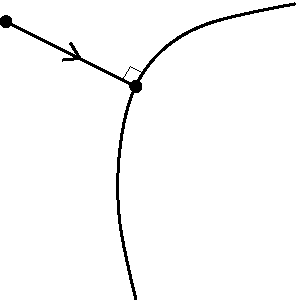
\includegraphics[height=40\unitlength]{closest}}
\cell{38}{38.5}{c}{$\hat{\p}$}
\cell{61.5}{27}{c}{$\p_\theta$}
\cell{64}{5}{c}{$(\p_\theta)_{\theta \in \Theta}$}
\end{picture}
\caption{Maximum likelihood and minimum relative entropy.}
\lbl{fig:rel-ent-max-like}
\end{figure}


\subsection*{Measure theory, geometry and statistics}

The connection between maximum likelihood and relative entropy involves
relative entropies $\relent{\hat{\p}}{\p_\theta}$ in which the arguments,
$\hat{\p}$ and $\p_\theta$, need not be close together in $\Delta_n$.
Nevertheless, we saw in the discussion of the Fisher metric that the
behaviour of $\relent{\p}{\vc{r}}$ when $\p$ and $\vc{r}$ are close is
especially significant.  More exactly, it is its infinitesimal behaviour to
second order that matters.  What follows is a brief further exploration of
this second-order behaviour, from a statistical perspective.

Let $\Omega$ be a measure space and let
$(f_\theta)_{\theta \in \Theta}$ be a smooth family of probability density
functions on $\Omega$, indexed over some real interval $\Theta$.  Fix
$\theta \in \Theta$.  The relative entropy
\[
\relent{f_\phi}{f_\theta} 
=
\int_\Omega f_\phi(x) \log \frac{f_\phi(x)}{f_\theta(x)} \dx
\]
($\phi \in \Theta$), defined as in
Example~\ref{egs:relent-meas}\bref{eg:rm-dens}, attains its minimum value
$0$ at $\phi = \theta$ (Figure~\ref{fig:fisher-curve}).
% 
\begin{figure}
\centering
\lengths
\begin{picture}(120,33)(0,-3)
\cell{60}{15}{c}{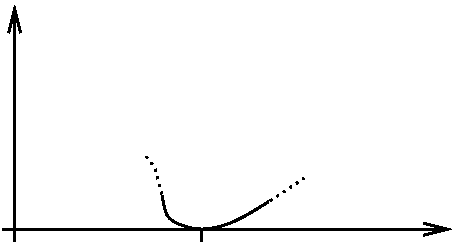
\includegraphics[height=30\unitlength]{locmin}}
\cell{23}{25}{c}{$\relent{f_\phi}{f_\theta}$}
\cell{56.5}{-0.5}{t}{$\theta$}
\cell{83}{-0.5}{t}{$\phi$}
\end{picture}
\caption{Relative entropy for a parametrized family of probability
  distributions.  The
  Fisher information $I(\theta)$ is the second derivative of the graph at
  $\theta$, that is, the curvature there.}
\lbl{fig:fisher-curve}
\end{figure}
% 
Thus, the function $\phi \mapsto \relent{f_\phi}{f_\theta}$ has both value
$0$ and first derivative $0$ at $\phi = \theta$.  The second derivative
measures how fast the distribution $f_\phi$ changes as $\phi$
varies near $\theta$.  It is called the
\demph{Fisher%
%
\index{Fisher, Ronald!information} 
% 
information} $I(\theta)$ of our family at $\theta$:
% 
\begin{equation}
\lbl{eq:fisher-info}
I(\theta)
=
\frac{\partial^2}{\partial\phi^2} \relent{f_\phi}{f_\theta} 
\biggr|_{\phi = \theta}.
\end{equation}
% 
Substituting the definition of $\relent{f_\phi}{f_\theta}$
into~\eqref{eq:fisher-info} and performing some elementary calculations
leads to an explicit formula for the Fisher information:
\[
I(\theta) 
= 
\int_\Omega 
\frac{1}{f_\theta} 
\biggl( \frac{\partial f_\theta}{\partial \theta} \biggr)^2.
\]

Detailed discussions of Fisher information can be found in texts such as
Amari and Nagaoka~\cite{AmNa} (Section~2.2), where the definition is given
for families of distributions parametrized by \emph{several} real variables
$\theta_1, \ldots, \theta_n$, and Fisher information is put into the
context of the Fisher metric.  Here, we simply describe two uses of Fisher
information in statistics, remaining in the single-parameter
case.

The first is the Cram\'er--Rao%
%
\index{Cramer, Harald@Cram\'er, Harald!Rao bound@--Rao bound}%
% \index{Cramer, Harald@Cram\'er, Harald}%
\index{Rao, C. Radhakrishna!Cram\'er--Rao bound}
%
bound.  Suppose that we have an unbiased estimator $\hat{\theta}$ of the
parameter $\theta$.  The \demph{Cram\'er--Rao bound} for $\hat{\theta}$ is
a lower bound on its variance:
% 
\begin{equation}
\lbl{eq:cr-bound}
\Var\bigl(\hat{\theta}\bigr) \geq \frac{1}{I(\theta)}
\end{equation}
% 
(Cram\'er~\cite{Cram}, Rao~\cite{RaoIAA}).

This statement can be understood as follows.  Let $\theta$ denote the true
but unknown value of our parameter, which we are trying to infer from the
data.  If the Fisher information $I(\theta)$ at $\theta$ is small, then
$f_\phi$ changes only slowly when $\phi$ is near $\theta$.  Different
parameter values near $\theta$ produce similar distributions, so it is
difficult to infer the parameter value from observations with any degree of
accuracy.  The Cram\'er--Rao bound~\eqref{eq:cr-bound} formalizes this
intuition: since $1/I(\theta)$ is in this case large, any unbiased
estimator of $\theta$ must be imprecise, in the sense of having large
variance.  In contrast, if $f_\phi$ varies rapidly near $\phi = \theta$
then inferring\index{inference} $\theta$ from the data is easier, and it
may be possible to find a more precise unbiased estimator.

A second use of Fisher information is in the definition of the Jeffreys
prior\index{prior}.  A fundamental challenge in Bayesian statistics is how
to choose a prior distribution on the parameter space $\Theta$.  In
particular, one can ask for a universal method that takes as its input a
family $(f_\theta)_{\theta \in \Theta}$ of probability distributions and
produces as its output a canonical distribution on
$\Theta$, intended to be used as a prior.  In 1939, the
statistician Harold%
%
\index{Jeffreys, Harold} 
% 
Jeffreys proposed using as a prior the density function
\[
\theta \mapsto \sqrt{I(\theta)},
\]
normalized (if possible) to integrate to $1$~\cite{JeffTP,JeffIFP}.  This is
the \demph{Jeffreys%
%
\index{Jeffreys, Harold!prior} 
% 
prior}.

The Jeffreys prior has the crucial property of invariance%
%
\index{invariance under reparametrization}
% 
under reparametrization.%
%
\index{reparametrization}
%  
For example, suppose that one person works with the family $(f_\sigma)_{0
  \leq \sigma \leq 10}$ of normal distributions on $\R$ with mean $0$ and
standard deviation between $0$ and $10$, while another works with the
family $(g_V)_{0 \leq V \leq 100}$ of normal distributions with mean $0$
and variance between $0$ and $100$.  The difference between the two
families is obviously cosmetic, and if calculations based on the different
parametrizations resulted in different outcomes, something would be
seriously wrong.

But the Jeffreys prior behaves correctly.  The first person
can calculate the Jeffreys prior of their family to produce a probability
density function on $[0, 10]$, hence a probability measure $\nu_1$ on $[0,
  10]$.  The second person, similarly, obtains a probability measure
$\nu_2$ on $[0, 100]$.  The invariance property is that when $\nu_1$ is
pushed forward along the squaring map $[0, 10] \to [0, 100]$, the resulting
measure on $[0, 100]$ is equal to $\nu_2$.  In other words, the choice of
parametrization makes no difference to the Jeffreys prior.  

This is a very important logical property, and not all systems for
assigning a prior possess it.  For instance, suppose that we simply
assign the uniform prior to any family (Bernoulli and Laplace's principle%
% 
\index{principle of insufficient reason}%
\index{insufficient reason, principle of}
% 
of insufficient reason, discussed in Section~3 of Kass and
Wasserman~\cite{KaWa}).  Then invariance fails: in the example above, a
probability of $1/2$ is assigned to the standard deviation being less than
$5$, but a probability of $1/4$ to the variance being less than $25$.  This
is a fatal flaw.

A careful account of the Jeffreys prior, with historical and mathematical
context, can be found in Section~4.7 of Robert, Chopin and
Rousseau~\cite{RCR}.  This includes the full multi-parameter definition,
extending the single-parameter version to which we have confined ourselves
here.


\section{Characterization of relative entropy}
\lbl{sec:rel-char}

Here we show that relative entropy is uniquely characterized by the four
properties listed in Section~\ref{sec:rel-defn}, proving:
% 
\begin{thm}
\lbl{thm:rel-char}
\index{relative entropy!characterization of}
% 
Let $\bigl(\melent{-}{-} \from A_n \to \R\bigr)_{n \geq 1}$ be a sequence
of functions.  The following are equivalent:
% 
\begin{enumerate}
\item 
\lbl{part:rel-char-props}
$\melent{-}{-}$ is measurable in the second argument,
permutation-invariant, and satisfies the vanishing and chain rules
(equation~\eqref{eq:rel-ch}, with $I$ in place of $H$);

\item
\lbl{part:rel-char-form}
$\melent{-}{-} = c\relent{-}{-}$ for some $c \in \R$.
\end{enumerate}
\end{thm}

Just as ordinary Shannon entropy has been the subject of many
characterization theorems, so too has relative entropy.
Theorem~\ref{thm:rel-char} and its proof first appeared in~\cite{SCRE}
(Theorem~II.1), and was strongly influenced by a categorical
characterization of relative entropy by Baez%
%
\index{Baez, John} 
%
and
Fritz~\cite{BaFr},%
%
\index{Fritz, Tobias}
%
which in turn built on work of Petz~\cite{Petz}.  It is also very close to
a result of Kannappan and Ng, although the proof is entirely different.
Historical commentary can be found in Remark~\ref{rmk:rel-char-hist}.

We now embark on the proof of Theorem~\ref{thm:rel-char}.

The four conditions in part~\bref{part:rel-char-props} are satisfied by
$\relent{-}{-}$ (as observed in Section~\ref{sec:rel-defn}), hence by
$c\relent{-}{-}$ for any scalar $c$.  Thus, \bref{part:rel-char-form}
implies~\bref{part:rel-char-props}.

\femph{For the rest of this section}, let $\melent{-}{-}$ be a sequence of
functions satisfying~\bref{part:rel-char-props}.  We have to prove that
$\melent{-}{-}$ is a scalar multiple of $\relent{-}{-}$.

Define a function $L \from (0, 1] \to \R$ by
\[
L(\alpha) = \melEnt{(1, 0)}{(\alpha, 1 - \alpha)}.
\]
(Since $\alpha > 0$, we have $\bigl((1, 0), (\alpha, 1 - \alpha)\bigr) \in
A_2$, so $L(\alpha) \in \R$ is well-defined.)  The idea is that if
$\melent{-}{-} = \relent{-}{-}$ then $L = -\log$. We will show that in
any case, $L$ is a scalar multiple of $\log$.

\begin{lemma}
\lbl{lemma:zeros}
Let $(\p, \vc{r}) \in A_n$ with $p_{k + 1} = \cdots = p_n = 0$, where $1
\leq k \leq n$.  Then $r_1 + \cdots + r_k > 0$ and
\[
\melent{\p}{\vc{r}} 
=
L(r_1 + \cdots + r_k) 
+
\melent{\p'}{\vc{r}'},
\]
where 
\[
\p' = (p_1, \ldots, p_k),
\qquad
\vc{r}' = \frac{(r_1, \ldots, r_k)}{r_1 + \cdots + r_k}.
\]
\end{lemma}

\begin{proof}
The case $k = n$ reduces to the statement that $L(1) = 0$, which follows
from the vanishing property.  Suppose, then, that $k < n$.  

Since $\p$ is a probability distribution with $p_i = 0$ for all $i > k$,
there is some $i \leq k$ such that $p_i > 0$, and then $r_i > 0$ since
$(\p, \vc{r}) \in A_n$.  Hence $r_1 + \cdots + r_k > 0$.  Let $\vc{r}'' \in
\Delta_{n - k}$ be the normalization of $(r_{k + 1}, \ldots, r_n)$ if $r_{k
  + 1} + \cdots + r_n > 0$, or choose $\vc{r}''$ arbitrarily in $\Delta_{n
  - k}$ otherwise.  (The set $\Delta_{n - k}$ is nonempty since $k < n$.)
Then by definition of composition,
% 
\begin{align*}
\p      &
= 
(1, 0) \of (\p', \vc{r}''),  \\
\vc{r}  &
= 
(r_1 + \cdots + r_k, \, r_{k + 1} + \cdots + r_n) \of (\vc{r}', \vc{r}'').
\end{align*}
% 
Hence by the chain rule, 
\[
\melent{\p}{\vc{r}}
=
L(r_1 + \cdots + r_k) +
1 \cdot \melent{\p'}{\vc{r}'} + 
0 \cdot \melent{\vc{r}''}{\vc{r}''},
\]
% 
and the result follows. 
\end{proof}

\begin{lemma}
\lbl{lemma:two-add}
$L(\alpha\beta) = L(\alpha) + L(\beta)$ for all $\alpha, \beta \in (0,
1]$. 
\end{lemma}

\begin{proof}
By the chain rule, $\melent{-}{-}$ has the logarithmic property stated at
the end of Section~\ref{sec:rel-defn} (equation~\eqref{eq:rel-log}, with
$I$ in place of $H$).  Hence
\[
\melEnt{(1, 0) \otimes (1, 0)}{(\alpha, 1 - \alpha) \otimes (\beta, 1 -
  \beta)}
=
L(\alpha) + L(\beta).
\]
But also
% 
\begin{align*}
&\melEnt{(1, 0) \otimes (1, 0)}%
{(\alpha, 1 - \alpha) \otimes (\beta, 1 - \beta)}       \\
&
=
\Melent{(1, 0, 0, 0)}%
{\bigl(\alpha\beta, \alpha(1 - \beta), 
(1 - \alpha)\beta, (1 - \alpha)(1 - \beta)\bigr)}       \\
&
=
L(\alpha\beta) + \melent{\vc{u}_1}{\vc{u}_1}    \\
&
=
L(\alpha\beta),
\end{align*}
% 
by Lemma~\ref{lemma:zeros} (with $k = 1$) and the vanishing property.  
\end{proof}

We can now deduce:

\begin{lemma}
\lbl{lemma:rel-two-log}
There is some $c \in \R$ such that $L(\alpha) = -c\log\alpha$ for all
$\alpha \in (0, 1]$.
\end{lemma}

\begin{proof}
By hypothesis, $L$ is measurable, so this follows from
Lemma~\ref{lemma:two-add} and Corollary~\ref{cor:cauchy-log-01}.
\end{proof}

Our next lemma is an adaptation of the most ingenious part of Baez and
Fritz's argument (Lemma~4.2 of~\cite{BaFr}).

\begin{lemma}
\lbl{lemma:bf-full-supp}
Let $n \geq 1$ and $(\p, \vc{r}) \in A_n$.  Suppose that $\p$ has full
support.  Then $\melent{\p}{\vc{r}} = c\relent{\p}{\vc{r}}$.
\end{lemma}

\begin{proof}
Since $(\p, \vc{r}) \in A_n$, the distribution $\vc{r}$ also has full
support.  We can therefore choose some $\alpha \in (0, 1]$ such that $r_i -
  \alpha p_i \geq 0$ for all $i$.

We will compute the number
\[
x =
\melEnt{(p_1, \ldots, p_n, \underbrace{0, \ldots, 0}_n)}
{(\alpha p_1, \ldots, \alpha p_n, 
r_1 - \alpha p_1, \ldots, r_n - \alpha p_n)} 
\]
in two ways.  (The pair of distributions on the right-hand side belongs to
$A_{2n}$, so $x$ is well-defined.)  First, by Lemma~\ref{lemma:zeros}
and the vanishing property,
\[
x 
=
L(\alpha) + \melent{\p}{\p}
=
-c\log\alpha.
\]
Second, by permutation-invariance and then the chain rule,
% 
\begin{align*}
x       &
=
\melEnt{(p_1, 0, \ldots, p_n, 0)}
{(\alpha p_1, r_1 - \alpha p_1, \ldots, \alpha p_n, r_n - \alpha p_n)} \\
&
=
\Melent{\p \of \bigl((1, 0), \ldots, (1, 0)\bigr)}
{\vc{r} \of 
\Bigl(
\Bigl(\alpha \tfrac{p_1}{r_1}, 1 - \alpha \tfrac{p_1}{r_1}\Bigr), \ldots, 
\Bigl(\alpha \tfrac{p_n}{r_n}, 1 - \alpha \tfrac{p_n}{r_n}\Bigr)
\Bigr)} \\
&
=
\melent{\p}{\vc{r}} + 
\sum_{i = 1}^n p_i L\Bigl(\alpha \tfrac{p_i}{r_i}\Bigr) \\
&
=
\melent{\p}{\vc{r}} - c\log \alpha - c\relent{\p}{\vc{r}}.
\end{align*}
% 
Comparing the two expressions for $x$ gives the result.
\end{proof}

We have now proved that $\melent{\p}{\vc{r}} = c\relent{\p}{\vc{r}}$ when
$\p$ has full support.  It only remains to prove it for arbitrary $\p$. 

\begin{pfof}{Theorem~\ref{thm:rel-char}}
Let $(\p, \vc{r}) \in A_n$.  By permutation-invariance, we can assume that 
\[
p_1, \ldots, p_k > 0, 
\quad
p_{k + 1} = \cdots = p_n = 0,
\]
where $1 \leq k \leq n$.  Writing $\rhow = r_1 + \cdots + r_k$,
\[
\melent{\p}{\vc{r}}     
=
L(\rhow) 
+ \melEnt{(p_1, \ldots, p_k)}{\tfrac{1}{\rhow}(r_1, \ldots, r_k)}
\]
by Lemma~\ref{lemma:zeros}.  Hence by Lemmas~\ref{lemma:rel-two-log}
and~\ref{lemma:bf-full-supp},
\[
\melent{\p}{\vc{r}}     
=
-c\log R
+ c\relEnt{(p_1, \ldots, p_k)}{\tfrac{1}{\rhow}(r_1, \ldots, r_k)}.
\]
But by the same argument applied to $cH$ in place of $I$ (or by direct
calculation), we also have
\[
c\relent{\p}{\vc{r}}     
=
-c\log R
+ c\relEnt{(p_1, \ldots, p_k)}{\tfrac{1}{\rhow}(r_1, \ldots, r_k)}.
\]
The result follows.
\end{pfof}

\begin{remarks}
\lbl{rmks:rel-char-hyps}
\begin{enumerate}
\item 
Cross entropy satisfies all the properties listed in
Theorem~\ref{thm:rel-char}\bref{part:rel-char-props} except for vanishing,
which it does not satisfy.  Hence the vanishing axiom cannot be dropped
from the theorem.

\item
\lbl{rmk:rel-char-hyps-ch}
The chain%
%
\index{chain rule!forms of} 
% 
rule can equivalently be replaced by a special case: 
% 
\begin{multline*}
\Melent{\bigl(pw_1, (1 - p)w_1, w_2, \ldots, w_n\bigr)}%
{\bigl(\widetilde{p}\widetilde{w}_1, (1 - \widetilde{p})\widetilde{w}_1, 
\widetilde{w}_2, \ldots, \widetilde{w}_n\bigr)}      \\ 
=
\melent{\vc{w}}{\widetilde{\vc{w}}} 
+
w_1 \melEnt{(p, 1 - p)}{(\widetilde{p}, 1 - \widetilde{p})}
\end{multline*}
% 
for all $(\vc{w}, \widetilde{\vc{w}}) \in A_n$ and $\bigl((p, 1 - p),
(\widetilde{p}, 1 - \widetilde{p})\bigr) \in A_2$.  Alternatively, it can
be replaced by a different special case:
% 
\begin{multline*}
\melEnt{w\p \oplus (1 - w)\vc{r}}%
{\widetilde{w}\widetilde{\p} \oplus (1 - \widetilde{w})\widetilde{\vc{r}}}%
\\
=
\melEnt{(w, 1 - w)}{(\widetilde{w}, 1 - \widetilde{w})}
+
w\melent{\p}{\widetilde{\p}}
+
(1 - w)\melent{\vc{r}}{\widetilde{\vc{r}}}
\end{multline*}
% 
for all $(\p, \widetilde{\p}) \in A_k$, $(\vc{r}, \widetilde{\vc{r}}) \in
A_\ell$, and $\bigl((w, 1 - w), (\widetilde{w}, 1 - \widetilde{w})\bigr)
\in A_2$.  Here we have used the notation
\[
w\p \oplus (1 - w)\vc{r}
=
\bigl(w p_1, \ldots, w p_k, (1 - w)r_1, \ldots, (1 - w)r_\ell\bigr).
\]
Both special cases are equivalent to the general case by elementary
inductions, as in Remark~\ref{rmk:ent-chain-simp} and
Appendix~\ref{sec:chain}.
\end{enumerate}
\end{remarks}

\begin{remark}
\lbl{rmk:rel-char-hist} 
% 
The first characterization of relative entropy appears to have
been proved by R\'enyi%
%
\index{Renyi Alfred@R\'enyi, Alfred} 
%
in 1961 (\cite{Reny}, Theorem~4).  It relied on $\relent{\p}{\vc{r}}$
being defined not only for probability distributions $\p$ and $\vc{r}$, but
also for all `generalized'%
%
\index{generalized probability distribution}%
\index{probability distribution!generalized}
%
distributions (in which
the requirement that $\sum p_i = \sum r_i = 1$ is weakened to $\sum p_i,
\sum r_i \leq 1$).  The result does not translate easily into a
characterization of relative entropy for ordinary probability distributions
only.

Among the theorems characterizing relative entropy for ordinary probability
distributions, one of the first was that of Hobson~\cite{Hobs}%
%
\index{Hobson, Arthur}
%
in~1969.  His hypotheses were stronger than those of
Theorem~\ref{thm:rel-char}, for the same conclusion.  In common with
Theorem~\ref{thm:rel-char}, he assumed permutation-invariance, vanishing,
and the chain rule (in the second of the two equivalent forms given in
Remark~\ref{rmks:rel-char-hyps}\bref{rmk:rel-char-hyps-ch}).  But he also
assumed continuity in both variables (instead of just measurability in one)
and a monotonicity hypothesis unlike anything in
Theorem~\ref{thm:rel-char}.

In 1973, Kannappan%
%
\index{Kannappan, Palaniappan}
%  
and Ng~\cite{KaNgMSF}%
%
\index{Ng, Che Tat}
%
proved a result very close to Theorem~\ref{thm:rel-char}.  They did not
explicitly \emph{state} that result in their paper, but the closing remarks
in another paper by the same authors~\cite{KaNgFEC} and the approach of a
contemporaneous paper by Kannappan and Rathie~\cite{KaRa} suggest
the intent.  The result resembling Theorem~\ref{thm:rel-char} was stated
explicitly in a 2008 article of Csisz\'ar (\cite{Csis}, Section~2.1), who
attributed it to Kannappan and Ng.

There are some small differences between the hypotheses of Kannappan and
Ng's theorem and those of Theorem~\ref{thm:rel-char}.  They assumed
measurability in both variables, whereas we only assumed measurability in
the second (and actually only used that $\melent{(1, 0)}{-}$ is
measurable).  On the other hand, they only needed the vanishing condition
for $\vc{u}_2$, whereas we needed it for all $\p$.  Like many authors on
functional equations in information theory, they used the chain rule in the
first of the equivalent forms in
Remark~\ref{rmks:rel-char-hyps}\bref{rmk:rel-char-hyps-ch}, under the name
of recursivity.

The proofs, however, are completely different.  Theirs was a tour de force
of functional equations, putting at its heart the so-called fundamental%
% 
\index{fundamental equation of information theory}
% 
equation of information theory (equation~\eqref{eq:feith}), and involving
the solution of such functional equations as
\[
f(x) + (1 - x) g\biggl( \frac{y}{1 - x} \biggr)
=
h(y) + (1 - y) j\biggl( \frac{x}{1 - y} \biggr)
\]
in four unknown functions.  The proof above bypasses these considerations
entirely. 
\end{remark}

